\documentclass[11pt]{amsbook}

\usepackage{../HBSuerDemir}	% ------------------------


\begin{document}

% ++++++++++++++++++++++++++++++++++++++
\hPage{b1p2/368}
% ++++++++++++++++++++++++++++++++++++++

Observe that the shaded region is not normal. If it is split up into $R_{xy}$ normal regions we get (at least) two such regions (AODB, ABEC). If it is split up into $R_{yx}$ normal regions we get (at least) three such regions (AODC, DBEC, BFE).
\begin{figure}[htbp]
	\centering
	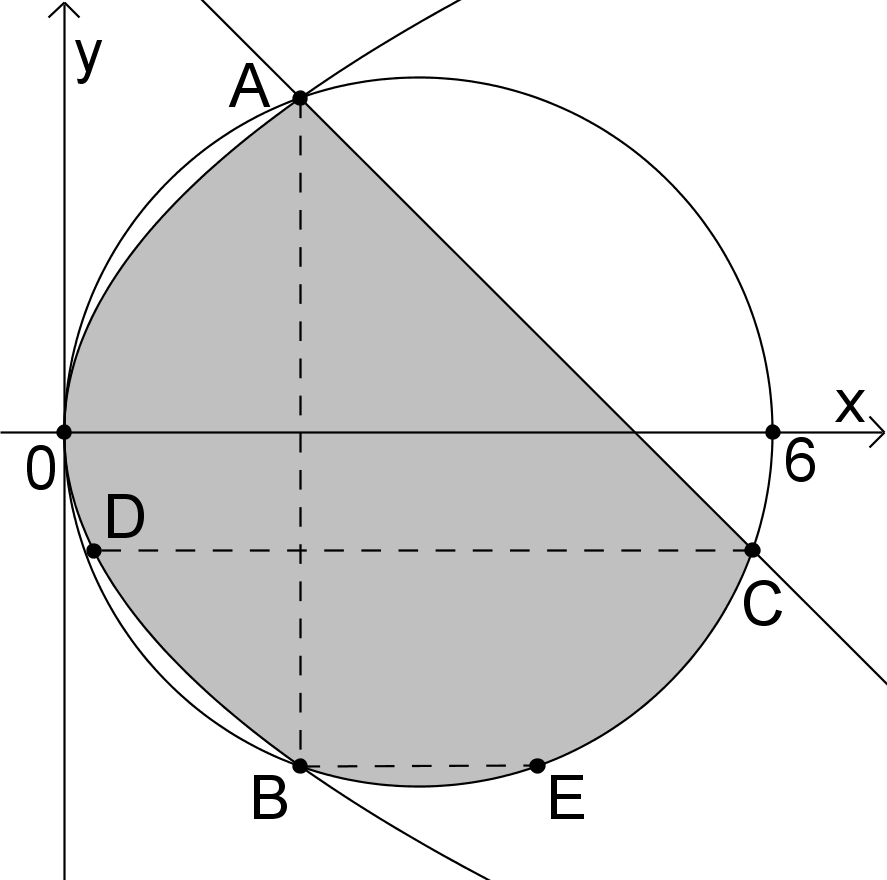
\includegraphics[width=0.4\columnwidth]{images/b1p2-368-fig01}
\end{figure}

It is reasonable to use the first splitting for this problem since the number of subregions is less than that of the other case. But in some problems such a selection may arise difficulty in integration.

Then our regions AODB, and ABEC are respectively:
\begin{align*}
	R_{xy}^{1} &= 
		\{ (x, y): 
		0 \leq x \leq 2,
		\ -2\sqrt{x} < y < 2\sqrt{x} \} 
		= (0,\ 2;
		\ -2\sqrt{x},\ 2\sqrt{x})  \\
	R_{xy}^{2} &= 
		\{ (x, y): 
		2 \leq x \leq 3+2\sqrt{2},
		\ -\sqrt{6x-x^{2}} \leq y \leq -x+2(1+\sqrt{2})\} \\
		& = (2,\ 3+2\sqrt{2};
		\ -\sqrt{6x-x^{2}},\ -x+2(1+\sqrt{2})) \\
	\hAbs{A} & = 
		\hAbs{R_{xy}^{1}}+\hAbs{R_{xy}^{2}} \\
	& = \int_{0}^{2} 
		(2\sqrt{x}-(-2\sqrt{x})) \, \hDif x 
		+\int_{2}^{3+2\sqrt{2}} 
			\!\!\! -x+2(1+\sqrt{2})-(-\sqrt{6x-x^{2}})) \, \hDif x \\
	& = \frac{16}{3} \sqrt{2} 
		+ \frac{7}{2} 
		+ \int_{2}^{3+2\sqrt{2}} 
			\sqrt{6x-x^{2}} \, \hDif x
\end{align*}
Writing $6x-x^{2}=9-(x-3)^{2}$ and setting $x-3=3\sin t$ we have
\begin{align*}
	\int \sqrt{6x-x^{2}} \, \hDif x 
	&= \int 
		\sqrt{9-9 \sin^{2} t} \cdot 3 \cos t \, \hDif t \\
	& = 9 \int 
		\cos^{2} t \, \hDif t 
	= \frac{9}{2} (t+ \frac{\sin 2t}{2}) + c \\
	\alpha = 
		\int_{2}^{3+2\sqrt{2}} 
			\sqrt{6x-x^{2}} \, \hDif x
	&= \frac{9}{2} \arcsin \frac{2 \sqrt{2}}{3} 
		+ \arcsin \frac{1}{3} + \frac{4 \sqrt{2}}{9}\\
	A = \frac{16}{3} \sqrt{2} + \frac{7}{2} + \alpha .
\end{align*}

% There must be
%
% \end{hSolution}
% \end{exmp}
%
% because the example and its solution is divided into two pages and i could 
% not write \end... without \begin{exmp} which must be in the previous page.


% ========================================
\end{document}  
